%!TEX root = manual.tex
%===============================================================================
\chapter{Real-time program}\label{ch:Assignment6}

The next version of the housekeeping program includes real-time requirements and the use of a real-time clock to add a timestamp to the housekeeping data sent to the ground station, simulated by the serial connection to the host PC like in the previous assignment. The hardware connections and the use of a host terminal application remain the same.

\section{Software architecture}

The software architecture now includes a period of 10 s for the {\tt TTC} task. This task reads the last value from the storage every 10 s (figure~\ref{fig:real-time}).

\begin{figure}[h]
            \centering{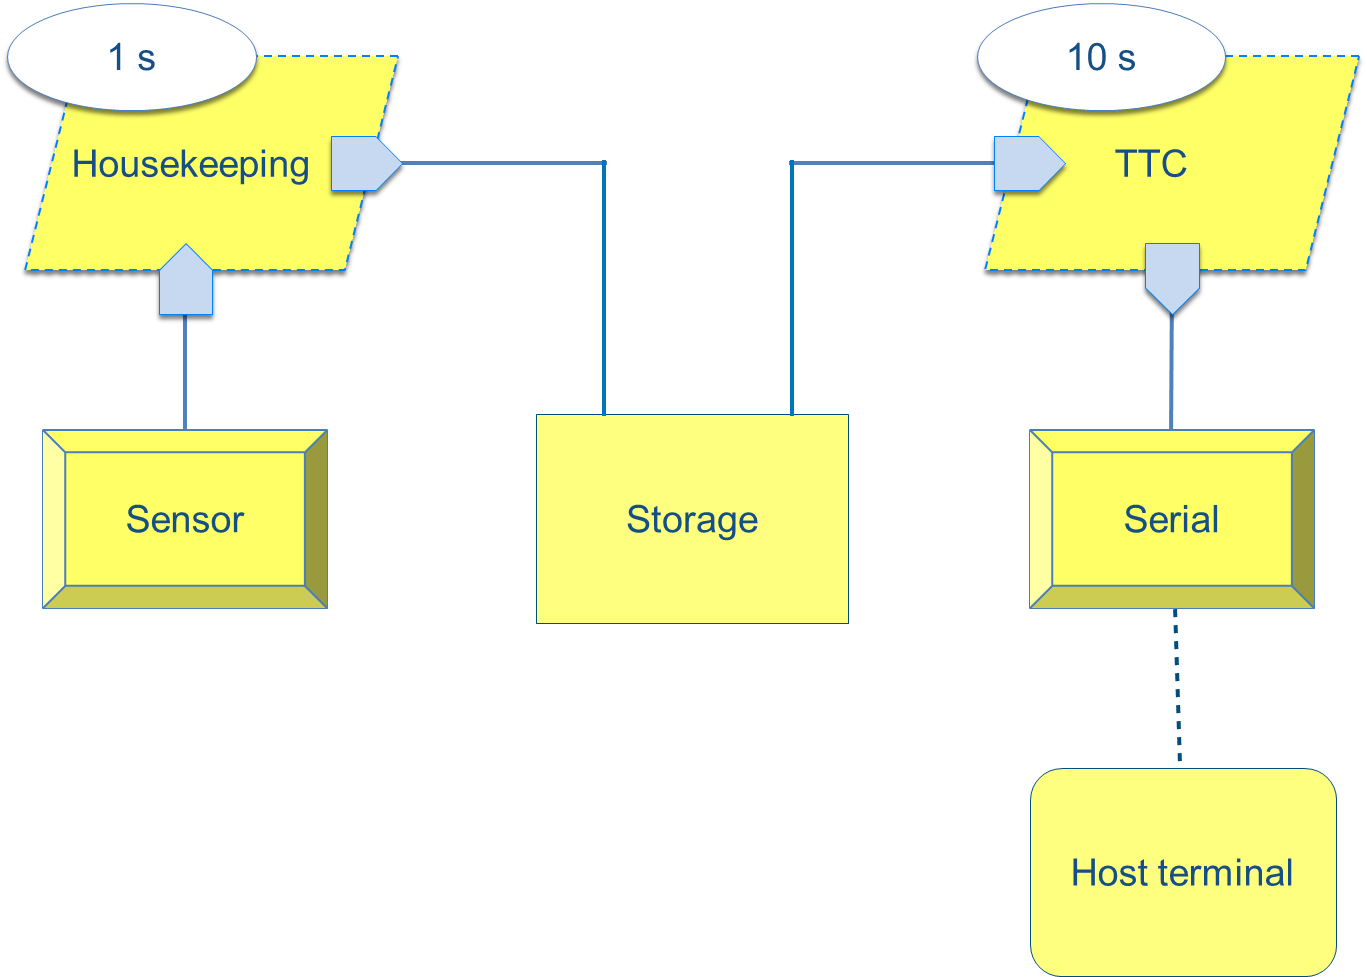
\includegraphics[width=0.8\textwidth,keepaspectratio]{real-time.png}}
            \caption{Software architecture of real-time housekeeping system.}
            \label{fig:real-time}
\end{figure}

\section{Real-time requirements}

The following real-time requirements are specified for the system:
\begin{itemize}
\item The {\tt Housekeeping} task executes with a period of 1 s and has a deadline equal to its period, (1 s).
\item The {\tt TTC} task executes with a period of 10 s and has a deadline of 2 s.
\end{itemize}

Priorities are assigned in deadline-monotonic order, as shown in table~\ref{tb:requirements}. The Buffer protected object, which is part of the {\tt Storage} implementation, is accessed by both application tasks and thus has a ceiling priority equal to the priority of the {\tt Housekeeping} task.

\begin{table}[htb]
\begin{center}
\begin{tabular}{|l|r|r|r|} \hline
Task & Period & Deadline & Priority\\ \hline
Housekeeping & 1.0 & 1.0 & 20 \\
TTC & 10.0 & 2.0 & 10 \\
Storage buffer & - & - & 20 \\ \hline
\end{tabular}
\caption{Real-time requirements.}
\label{tb:requirements}
\end{center}
\end{table}

\section{Download the code and study the implementation.}

The implementation code, as initially provided to the students, can be downloaded from \url{https://github.com/STR-UPM/OBDH\_LABS}. Click on {\tt Clone} or {\tt download}, download a zip archive, unzip and move to your work directory. The code for this assignment is in the LAB6 folder.

The implementation code differs from the previous project in several aspects.
\begin{itemize}
\item Period and priority values have been explicitly added to the specification of the {\tt Housekeeping} and {\tt TTC} packages. A start delay has been added to the respective tasks, in order to let all the packages initialize before the regular operation of the system starts.
\item The ceiling priority of the {\tt Storage} buffer has been set to the same value as the {\tt Housekeeping} task.
\item A new {\tt State} data type has been defined, which is a record including a timestamp and an analog data value. Messages sent to ground are now of this data type.

Timestamps are refined as 64-bit integers, denoting the number of second elapsed since the beginning of the mission. To the purpose of this laboratory this value is taken from the real-time clock provided by the {\tt Ada.Real\_Time} library package.
\item In order to improve the visual aspect of the messages as viewed on the host terminal application, a new package, {\tt Data\_Images}, has been added that provides fixed-width string images of mission time and analog data values.
i\end{itemize}

The rest of the implementation is the same as in the previous project.

\section{Compile and run.}

Open GPS and do the following:
\begin{enumerate}
\item Select {\tt Open} project on the welcome window. Navigate to the LAB6 directory and open the {\tt realtime\_housekeeping.gpr} project file.
\item Build the executable and load it into the board by clicking on the \hbox{
\includegraphics[width=1.5em]{buildandload.png}} symbol in the tool bar (or select {\tt Build} $\rightarrow$ {\tt Bareboard} $\rightarrow$ {\tt Flash to board} on the top menu).

The program will be compiled, and the executable will be loaded into the board flash memory. After that, the program starts to run on the board (check the blinking LEDs).
\item Connect the serial cable to a USB port on the host computer, if not already done.
\item Identify the serial port name on the host computer and launch the remote terminal application as explained in section~\ref{sc:term}.  The sensor measured values together with their respective timestamps will start being displayed on the host application (figure~\ref{fig:output}).
\end{enumerate}

\begin{figure}[h]
            \centering{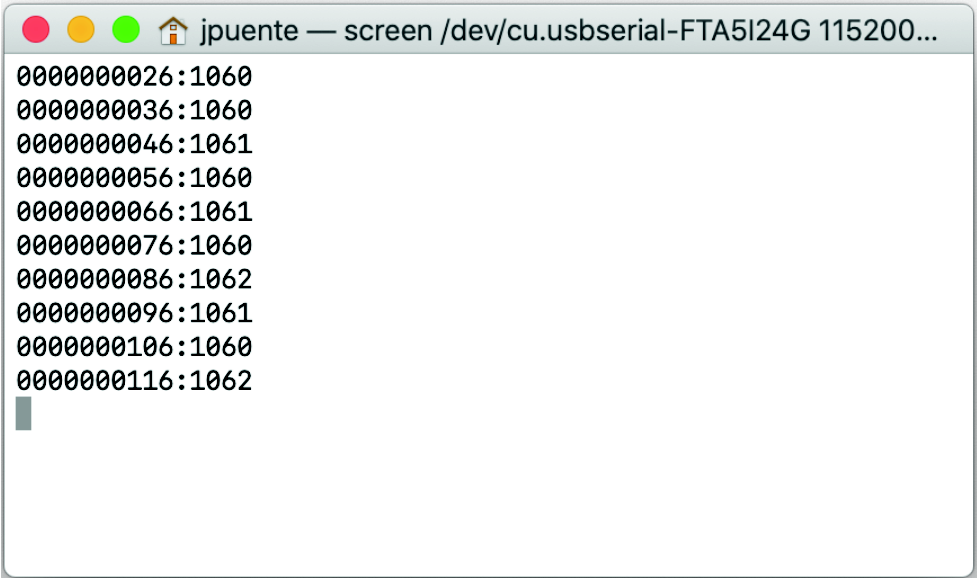
\includegraphics[width=0.6\textwidth,keepaspectratio]{output.png}}
            \caption{Sample output on host terminal.}
            \label{fig:output}
\end{figure}

\section{Perform a temporal analysis of the system.}\label{sc:ta}

In order to carry out a response-time analysis of the temporal behaviour of the system, you will need to measure the execution time of the task bodies and the protected procedure bodies. A simple loop technique using the standard real-time clock will be enough for this assignment.

An execution time measurement tool is available in the LAB6 directory. In order to use it, perform the following steps:
\begin{enumerate}
\item Open GPS and select {\tt Open} project on the welcome window. Navigate to the LAB6 directory and open the {\tt wcet\_meter.gpr} project file.
\item Build the executable and load into the board in the same way as for the realtime\_housekeeping.gpr project.
\item Make sure that the serial cable is still connected to the board and the USB port in the host computer. If the remote terminal application is not open, open it.
\end{enumerate}

A measurement test is executed on the board, and repeated every 60 s. The output of the test is shown on the host terminal application (figure~\ref{fig:wcet}). The output shows the execution times for the bodies of the {\tt Housekeeping} (HK) and {\tt TTC} (TC) tasks, as well as the bodies of the protected operations of the {\tt Storage} object (ST). Notice that a new entry, {\tt Get\_Immediate}, has been added for the latter in order to avoid the measuring task to get blocked. The new entry is exactly the same as {\tt Get} but has a {\tt True} barrier so that it is always open.

\begin{figure}[h]
            \centering{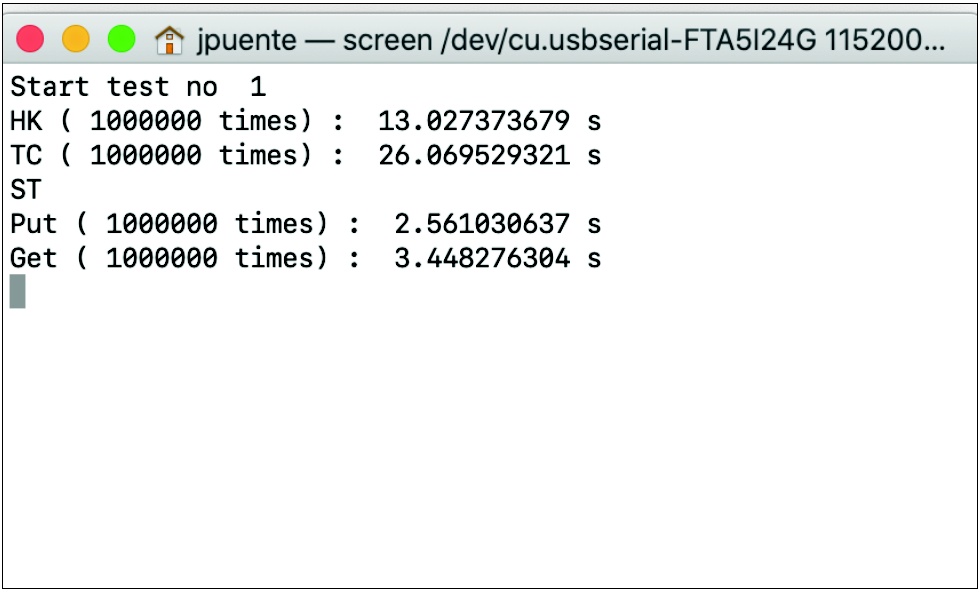
\includegraphics[width=0.6\textwidth,keepaspectratio]{wcet.png}}
            \caption{Output of wcet measurement tool.}
            \label{fig:wcet}
\end{figure}

In the example shown on figure~\ref{fig:wcet}, the HK execution time has been measured $10^{6}$ times, with a total measurement time of 13.02 s. Therefore, the value to be taken for the response time analysis is $13.02\cdot10^{-6}~s = 13.02~\mu${s}, and the same for the other tasks. Take into account that the values measured on your board will probably be slightly different from the above shown.

Once you have an estimate of worst case execution times, apply the RTA equations for computing the worst-case response time and check if all the deadlines are met. The setup for the calculations is shown on table~\ref{tb:wcet}.

\begin{table}[htb]
\begin{center}
\begin{tabular}{|l|r|r|r|r|r|r|r|r|} \hline
Task & T & C & B & D & R & P & Storage & Operation\\ \hline
Housekeeping & 1.0 & $13\cdot10^{-6}$ & $4\cdot10^{-6}$ & 1.0 & $17\cdot10^{-6}$& 20 & $3\cdot10^{-6}$ & CPut \\
TTC & 10.0 & $26\cdot10^{-6}$ & 0 & 2.0 & $39\cdot10^{-6}$ & 10 & $4\cdot10^{-6}$ & CGet \\ \hline
& & & & & & CP & \multicolumn{2}{|c|}{20} \\ \hline
\end{tabular}
\caption{Data arrangement for RTA of the housekeeping system.}
\label{tb:wcet}
\end{center}
\end{table}
